\documentclass[12pt]{article}
\usepackage{fancyvrb}
\usepackage{graphicx}
\usepackage{mathptmx}
\usepackage{etoolbox}
\usepackage{ragged2e}
\usepackage{tabularx}
\usepackage{hyperref}
\usepackage{geometry}
\usepackage{etoolbox}
\usepackage{float}
\usepackage[acronym]{glossaries}
\makeatletter
% \patchcmd{<cmd>}{<search>}{<replace>}{<success>}{<failure>}
\patchcmd{\@makechapterhead}{\huge}{\large}{}{}% for \chapter
\patchcmd{\@makechapterhead}{\Huge}{\large}{}{}% for \chapter
\patchcmd{\@makeschapterhead}{\Huge}{\large}{}{}% for \chapter*
\tolerance=1
\emergencystretch=\maxdimen
\hyphenpenalty=10000
\hbadness=10000
\geometry{a4paper,total={170mm,257mm},left=20mm,top=20mm}

\patchcmd{\thebibliography}{\section*{\refname}}{}{}{}

\begin{document}
\begin{titlepage}
    \centering
    
\includegraphics[width=10cm]{manipal.png}
    
    \vskip7.4cm
    ITT Lab Report\\
    B.Tech IT 6$^{th}$ Semester\\
    \vskip1cm
    {\bfseries\Large
        PopResumé: A Resumé builder web app\\
    }
    \vskip1cm
    \textit{Submitted by}
    \vskip0.5cm
    \begin{tabularx}{0.8\textwidth} {>{\raggedright\arraybackslash}X>{\raggedleft\arraybackslash}X}
        Siddhant Dorman & 180911142 \\
        Nikesh Kumar & 180911202 \\
        Anjali Singh & 180911274
    \end{tabularx}
    \vfill
\end{titlepage}

\tableofcontents
\thispagestyle{empty}
\newpage

\justify
% ---------------- Introduction ----------------
\pagenumbering{arabic}
\section*{\LARGE{Introduction}}
\addcontentsline{toc}{section}{\protect\numberline{}Introduction}
This project aims to build an intuitive online platform for building resumes for individuals. The web app will be flexible, interactive and will reduce the need to think and design an appropriate resume according to qualifications. It will provide an easy means for creating a professional-looking resume. Individuals will have to fill up a form that will include information like educational qualification, work experience, interest, skills, etc. The user will have various resume template options to choose from depending on their job profile. 
% \newpage

% ---------------- Framework and Database Description ----------------
\section*{\LARGE{Framework and Database Description}}
\addcontentsline{toc}{section}{\protect\numberline{}Framework and Database Description}
We used the \textbf{PERN} stack to deploy the project, which stands for Postgres, Express, React, NodeJS.
The front-end was designed on \textbf{React JS} for component-based development of the main landing page, login module, and so on.
The front-end communicates with the backend served by \textbf{Express}. The Express backend makes use of OAuth provided by Google as well as our Login System which makes usage of JWT (JSON Web Token) to establish sessions.
For the database, Sequelize Package communicates with \textbf{PostgreSQL}, which is a relational database. React JS and Express, both are frameworks that run in \textbf{Node JS} environment.

\begin{figure}[H]
\centering
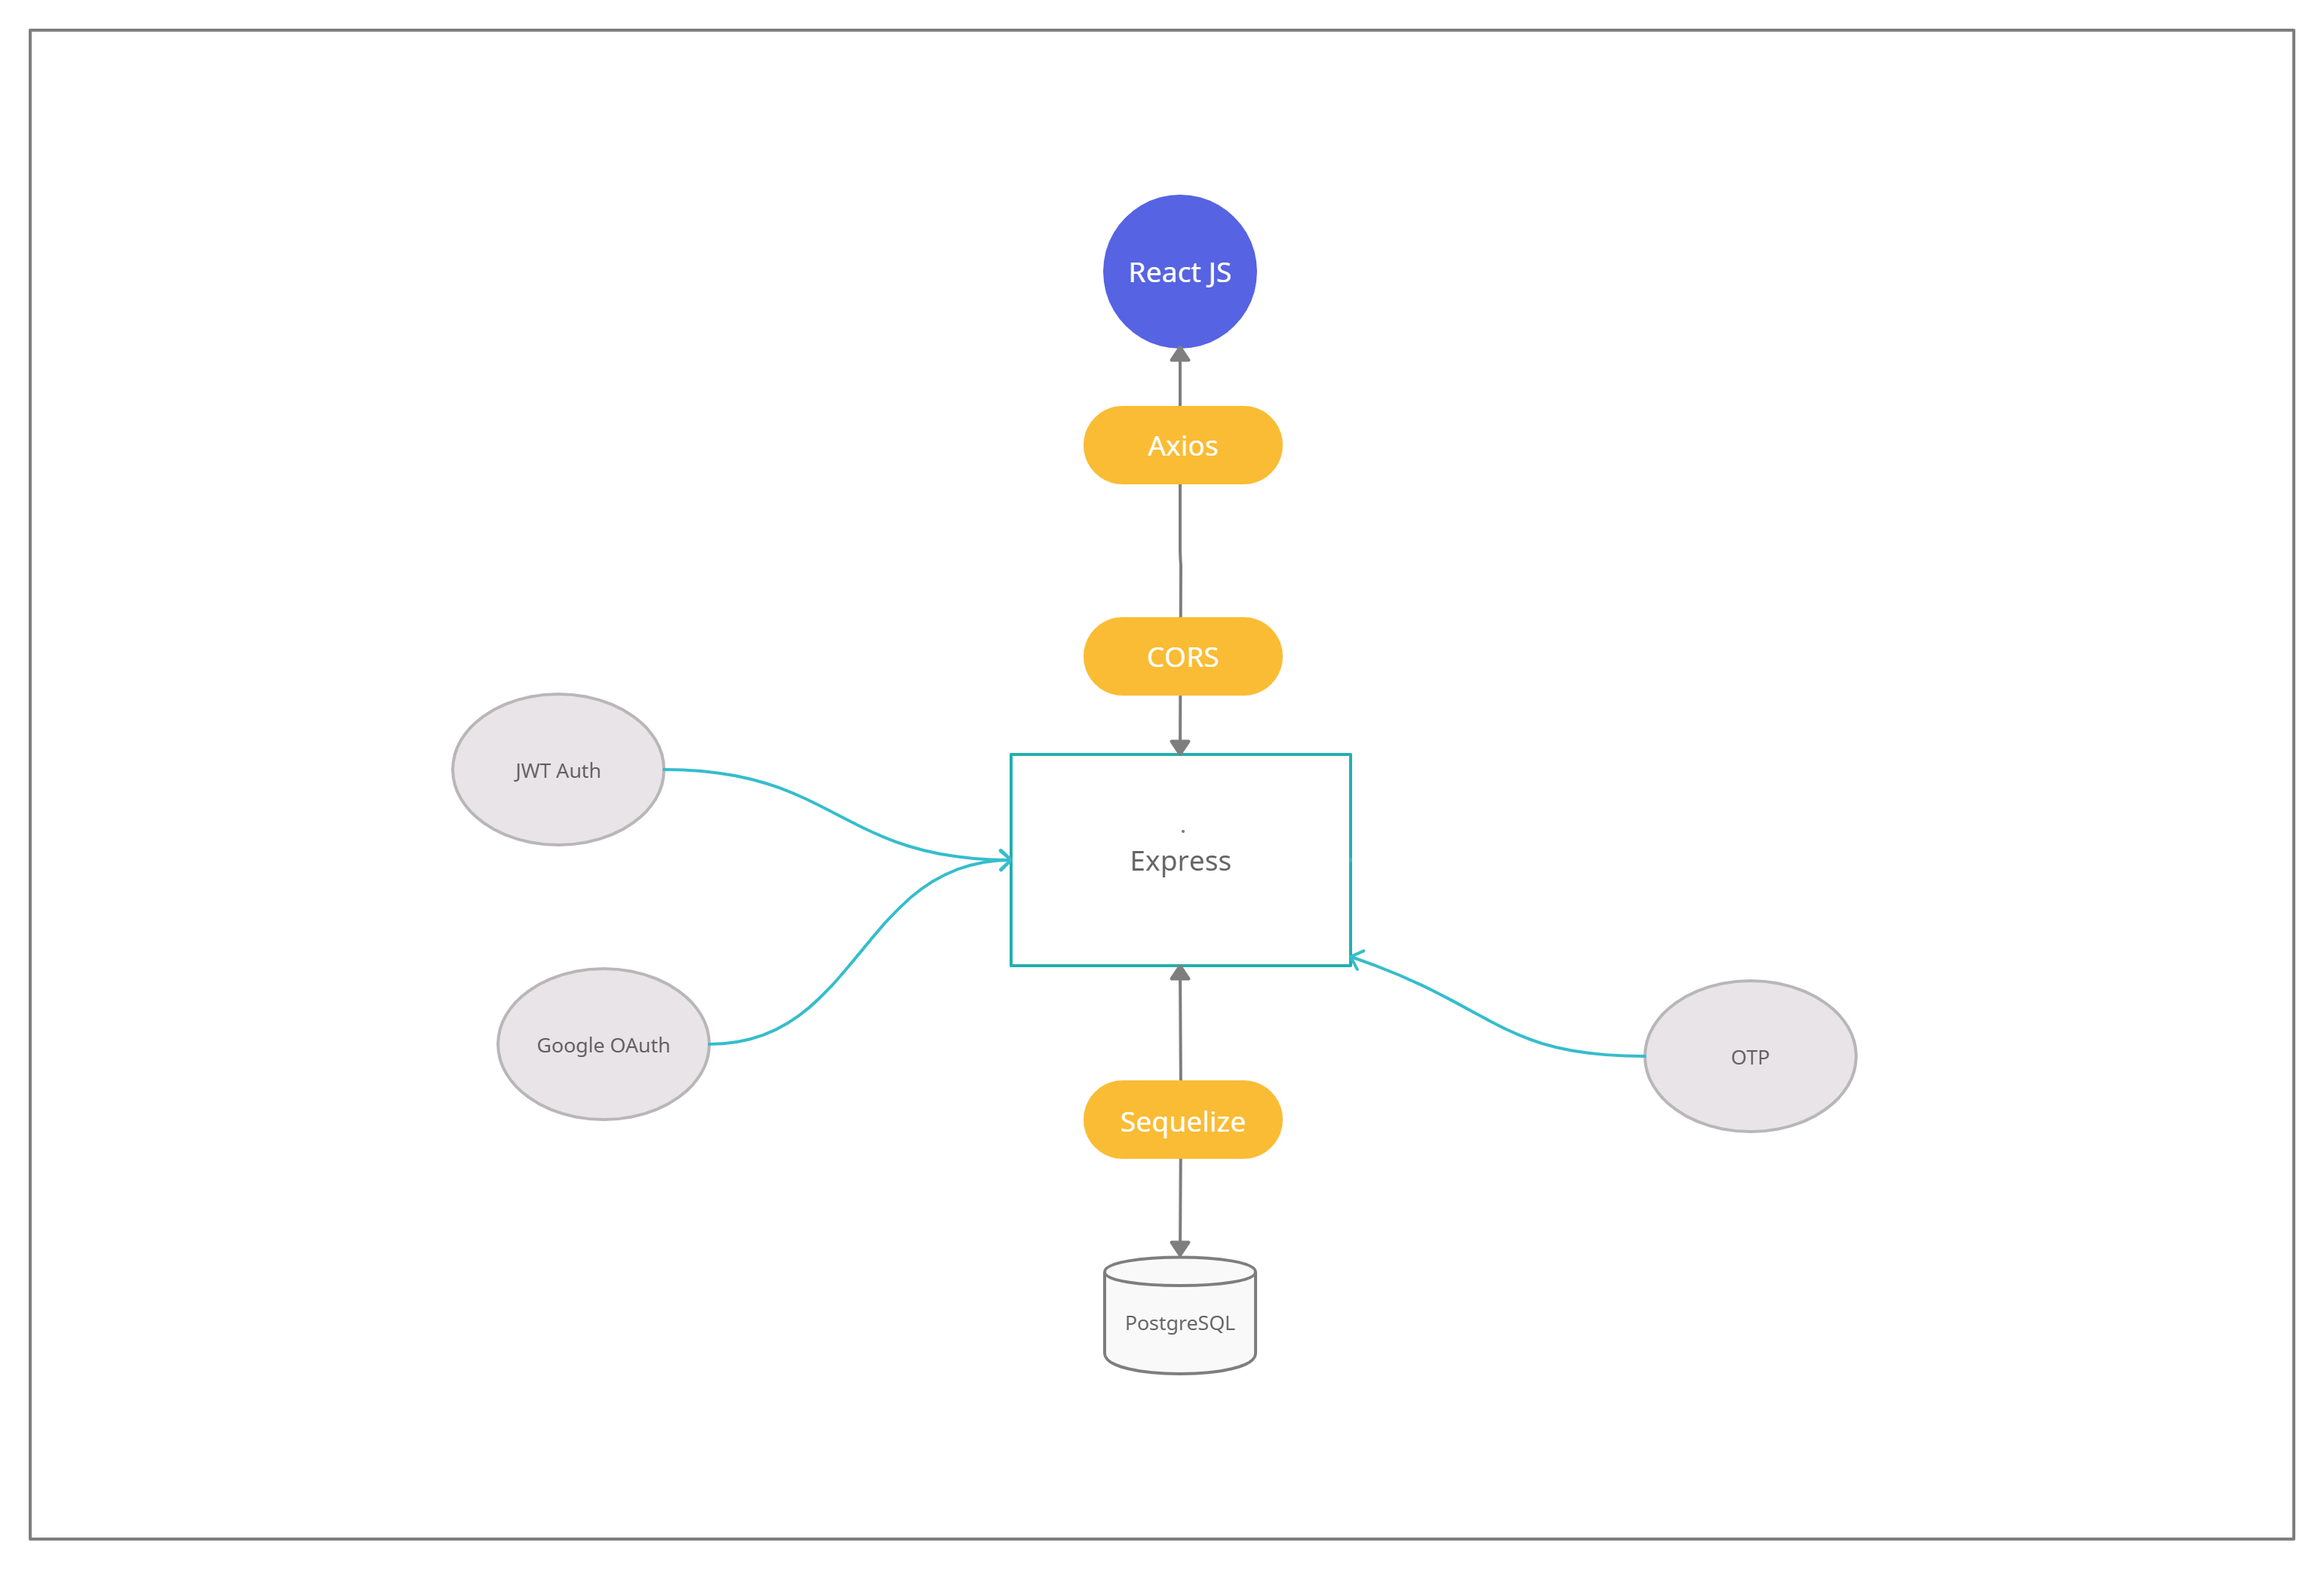
\includegraphics[width=\linewidth]{diagram.png}
\caption{Flowchart}
\end{figure}

\newpage

% ---------------- Implementation Details ----------------
\section*{\LARGE{Implementation Details}}
\addcontentsline{toc}{section}{\protect\numberline{}Implementation Details}

\subsection*{\Large{Frontend}}
\addcontentsline{toc}{subsection}{\protect\numberline{}Frontend}

The frontend has been built on React JS which is compiled to give a minified version containing the HTML, CSS \& JS that is then served by the backend. In many cases, the frontend can also be deployed on a different domain given that the backend allows cross-origin access from that particular domain. The frontend has primarily 3 Routes:

\subsubsection*{Home}
\addcontentsline{toc}{subsubsection}{\protect\numberline{}Home}
The Home Route handles the landing of any user and introduces them to the application. This makes use of another component called \textit{Resume} which is the component for Resume editing but here it shows how a resume works in PopResume. That aside, the user has an option to head to the log in page or register page from this route.

\subsubsection*{Login}
\addcontentsline{toc}{subsubsection}{\protect\numberline{}Login}
The Login Route handles user login/signup which can be toggled by clicking the thinking emoji.\par The login side has 2 options where a registered user can login or directly sign in via Google Account instead. After successful sign up the user is sent to ResumeHandler, and in case of failure, an appropriate message is shown.\par The register side has 2 phases. The first part is where the user fills a form and a check is performed to verify if the user is valid. If successful, an OTP is generated that expires in $7 min$ and is sent to the user, else an appropriate error is notified. The user can either enter the OTP directly and get verified or click on the URL sent and automatically get verified.\par Furthermore, animations have been added to the page for a fluid look with the help of \textit{GSAP} and \textit{TweenMax}.

\subsubsection*{ResumeHandler}
\addcontentsline{toc}{subsubsection}{\protect\numberline{}ResumeHandler}
This is where the core functionality of our app lies. The user will make changes to the form having options for different sections, changing themes, details, layout, etc. The document could then be downloaded by the user as a PDF or saved to the database.

\subsection*{\Large{Backend}}
\addcontentsline{toc}{subsection}{\protect\numberline{}Backend}

The backend has been built on the Express framework and makes use of a relational DB called PostgreSQL for storage purposes, which has been synced with the app using the Sequelize package. The Express app makes use of CORS package to communicate across different origins. JWT has been used to establish a user's identity and for easy communication. A route is mounted on `api/user' that handles all user related procedures such as authentication, login, signup, OTP generation, verification. Means have been provided for backend to emit an event in case of OTP verification via link. The backend has a login system for users and an OTP system the clears data after a given interval with the structure given below.

\begin{Verbatim}[frame=single]
client(id TEXT,fname TEXT,lname TEXT,pwd TEXT,link_gmail BOOLEAN,
img_thumb TEXT);
otp (id uuid,email_id TEXT,expiry DATE,otp CHAR(6));
\end{Verbatim}

% \newpage

% ---------------- Screenshots ----------------
\section*{\LARGE{Screenshots}}
\addcontentsline{toc}{section}{\protect\numberline{}Screenshots}

\begin{figure}[H]
\centering
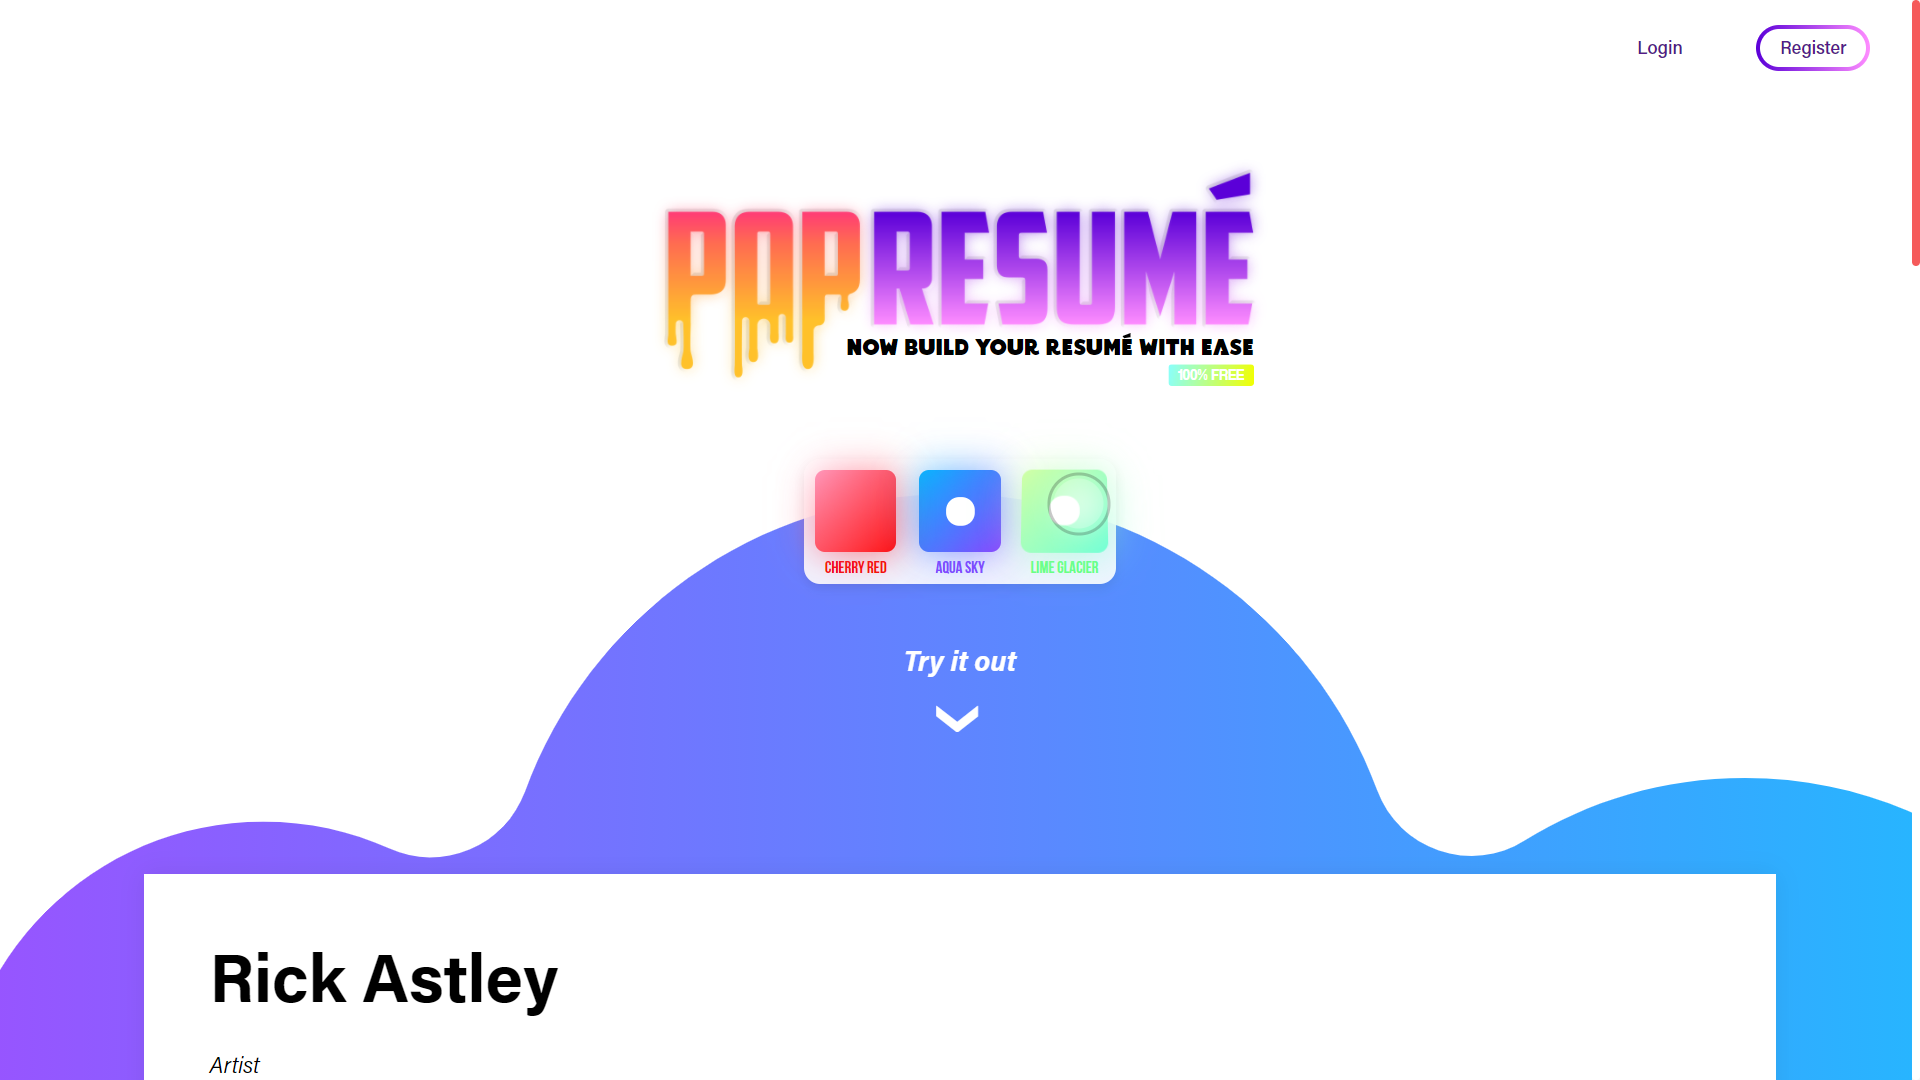
\includegraphics[width=0.7\linewidth]{Screenshot (123).png}
\caption{Main Landing Page}
\end{figure}
\begin{figure}[H]
    \begin{minipage}{0.47\textwidth}
        \centering
        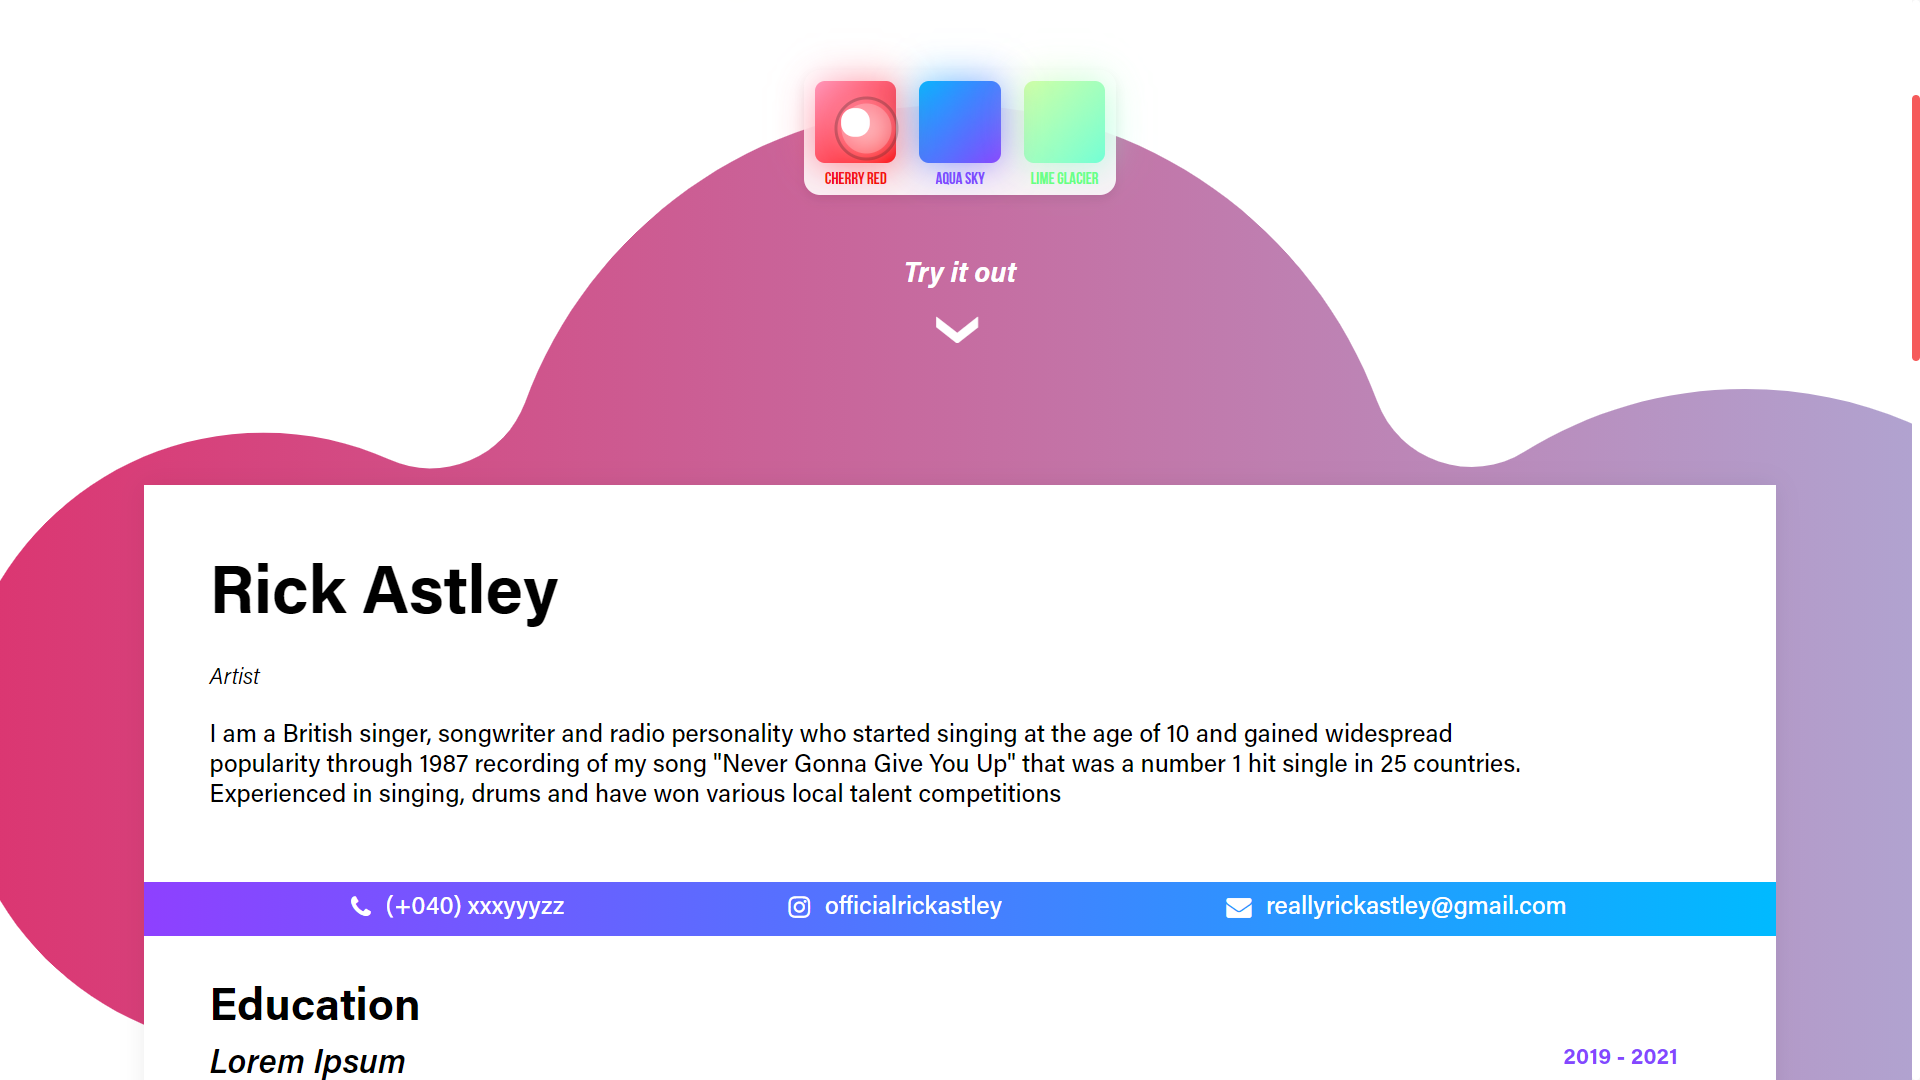
\includegraphics[width=\linewidth]{Screenshot (124).png}
        \caption{Main Landing Transition Begin}
    \end{minipage}\hfill
    \begin{minipage}{0.47\textwidth}
        \centering
        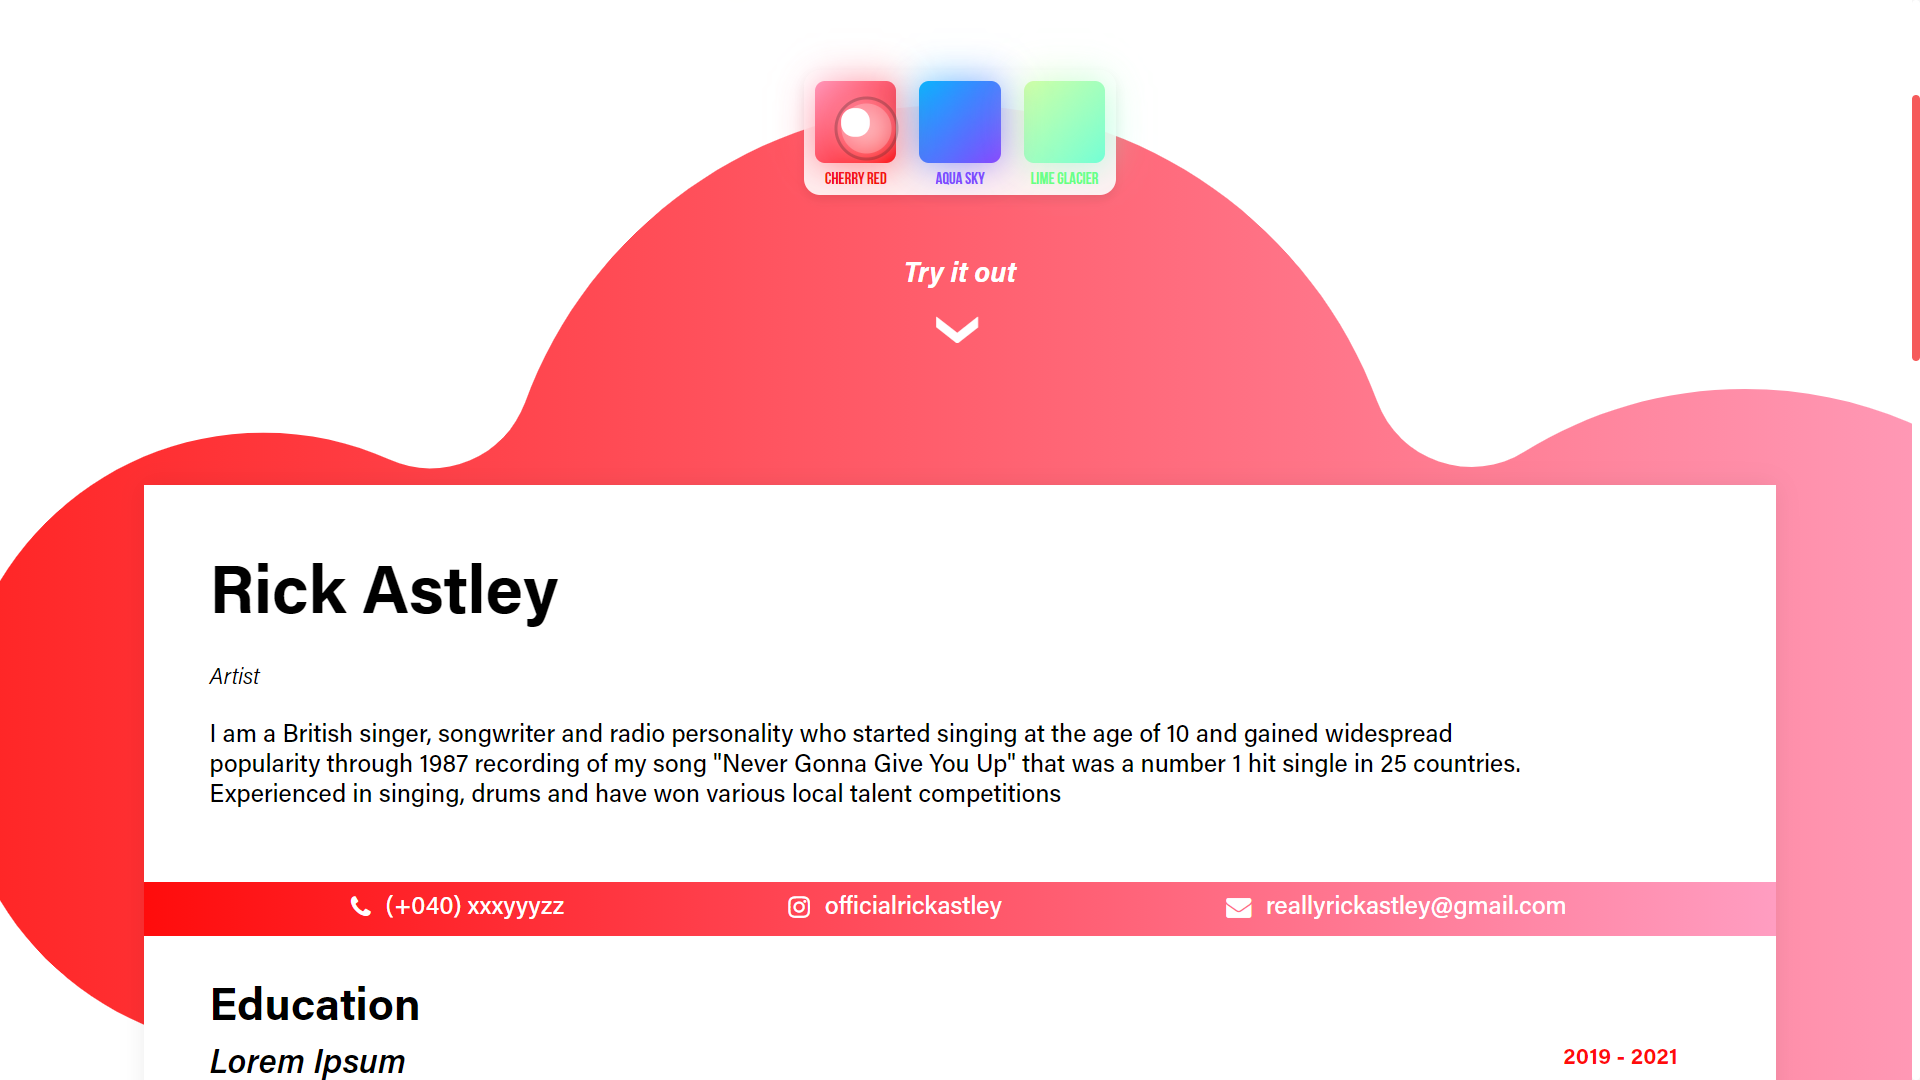
\includegraphics[width=\linewidth]{Screenshot (125).png}
        \caption{Main Landing Transition End}
    \end{minipage}
\end{figure}
\begin{figure}[H]
\centering
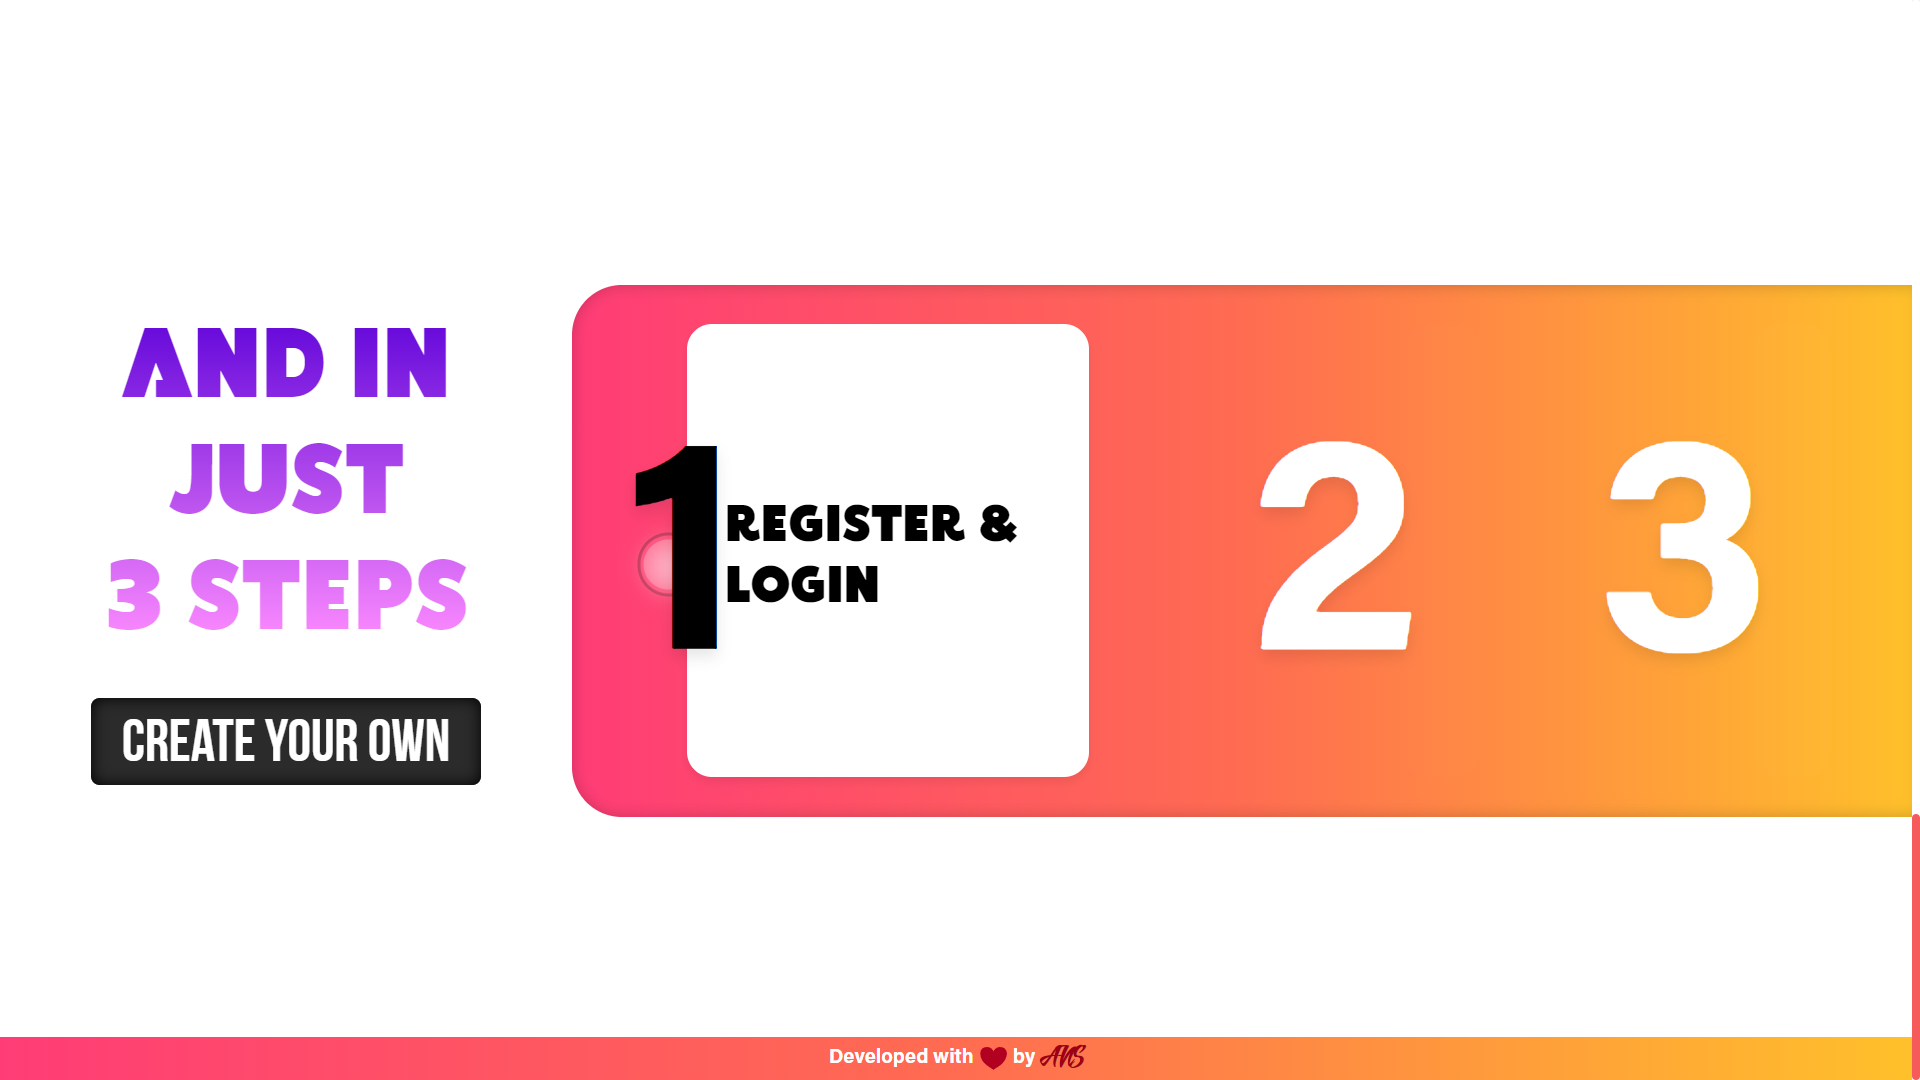
\includegraphics[width=0.7\linewidth]{Screenshot (127).png}
\caption{Main Landing Page - Bottom Part}
\end{figure}

\begin{figure}[H]
\centering
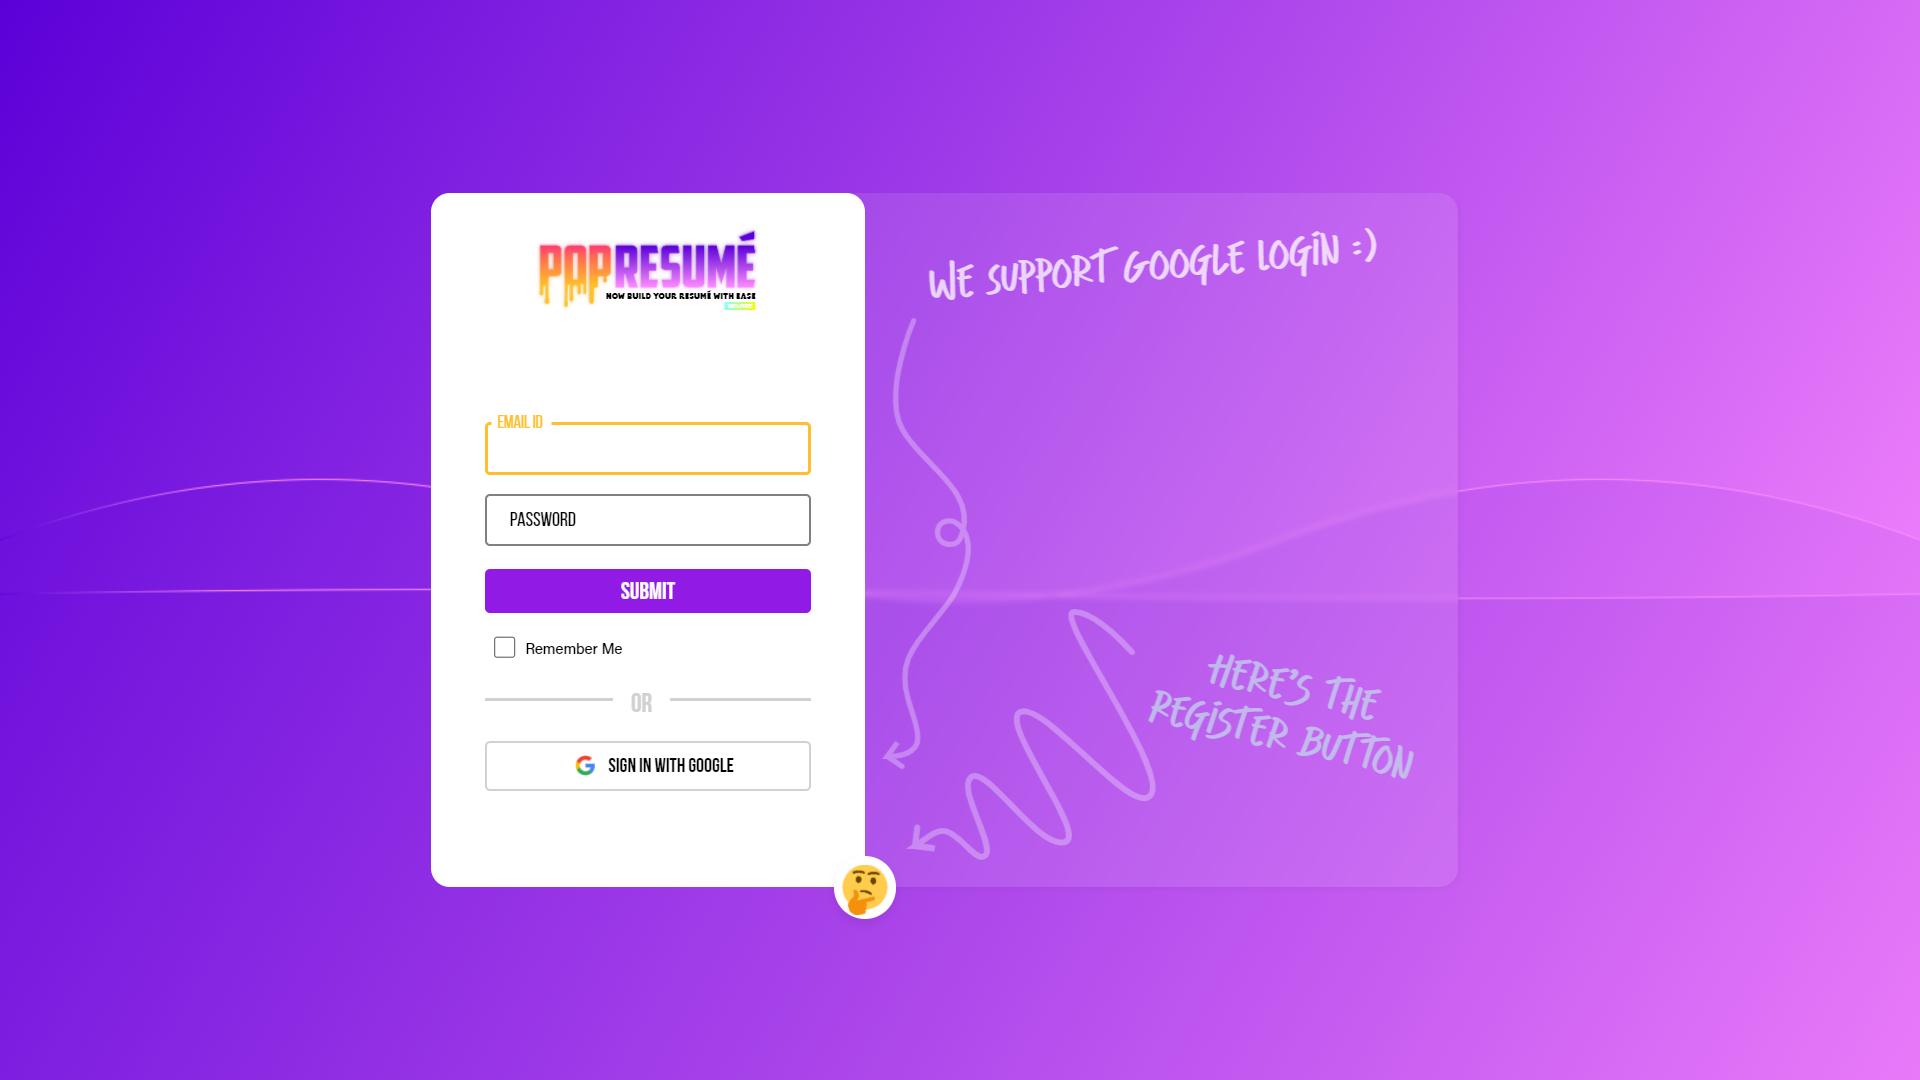
\includegraphics[width=0.7\linewidth]{Screenshot (129).png}
\caption{Login Page}
\end{figure}
\begin{figure}[H]
    \begin{minipage}{0.47\textwidth}
        \centering
        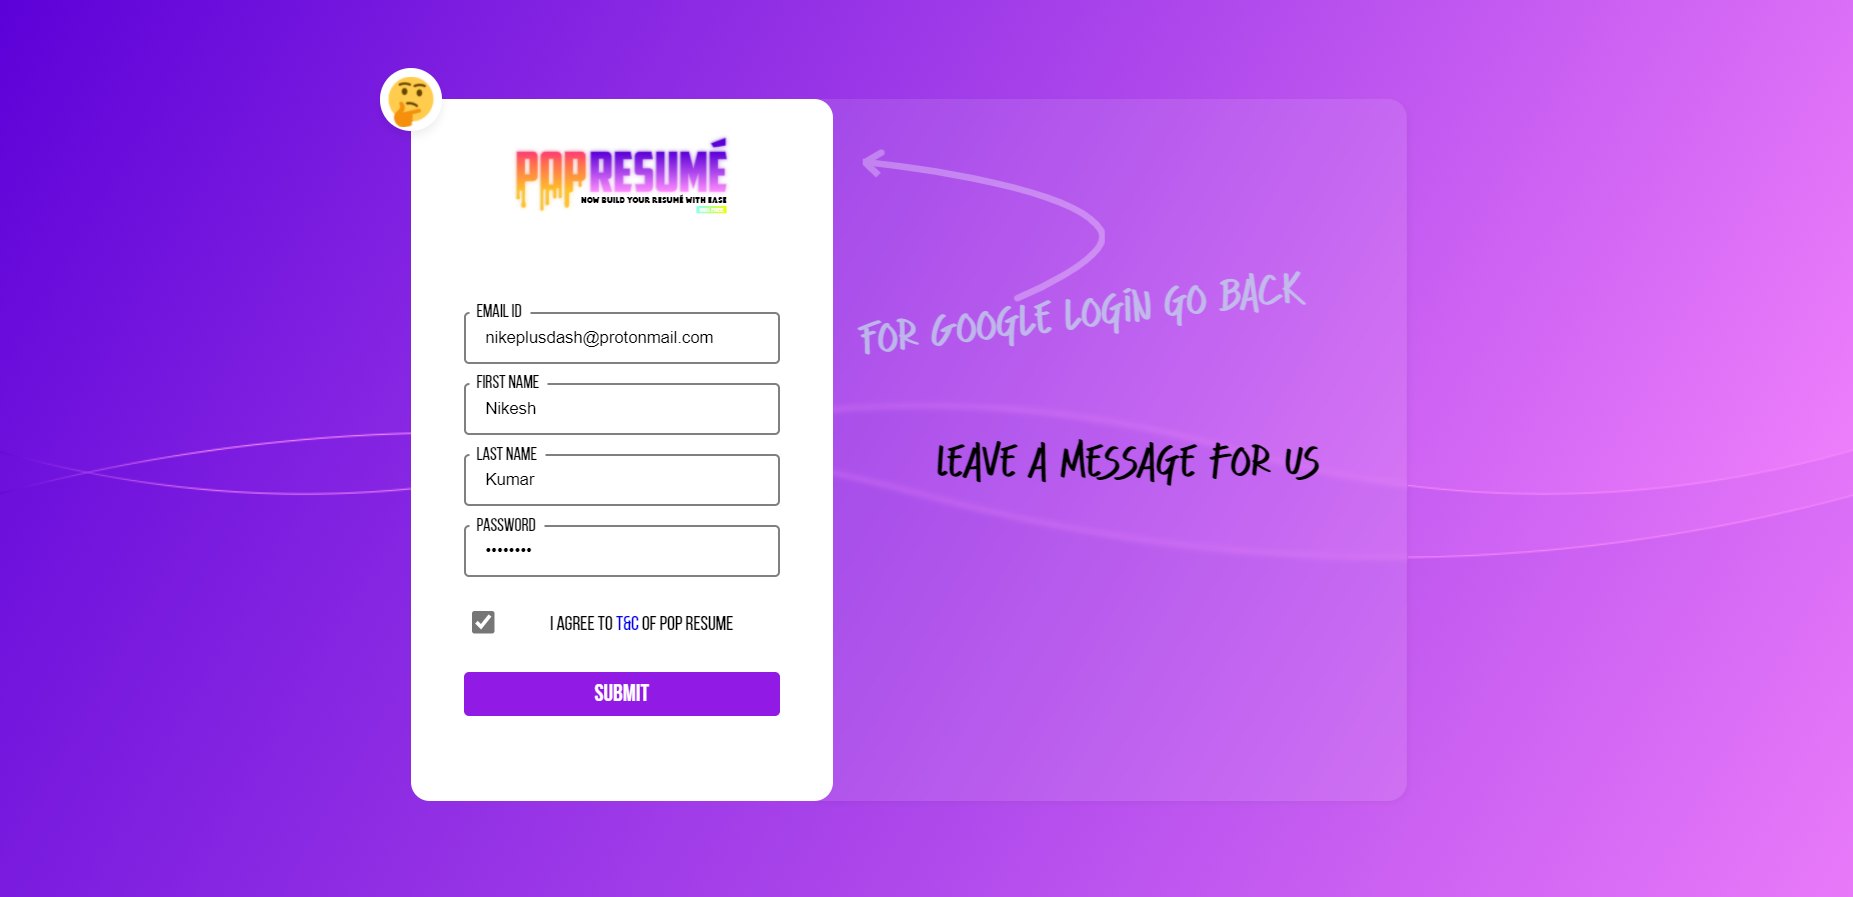
\includegraphics[width=\linewidth]{Screenshot 2021-06-07 051600.png}
        \caption{Registration Page}
    \end{minipage}\hfill
    \begin{minipage}{0.47\textwidth}
        \centering
        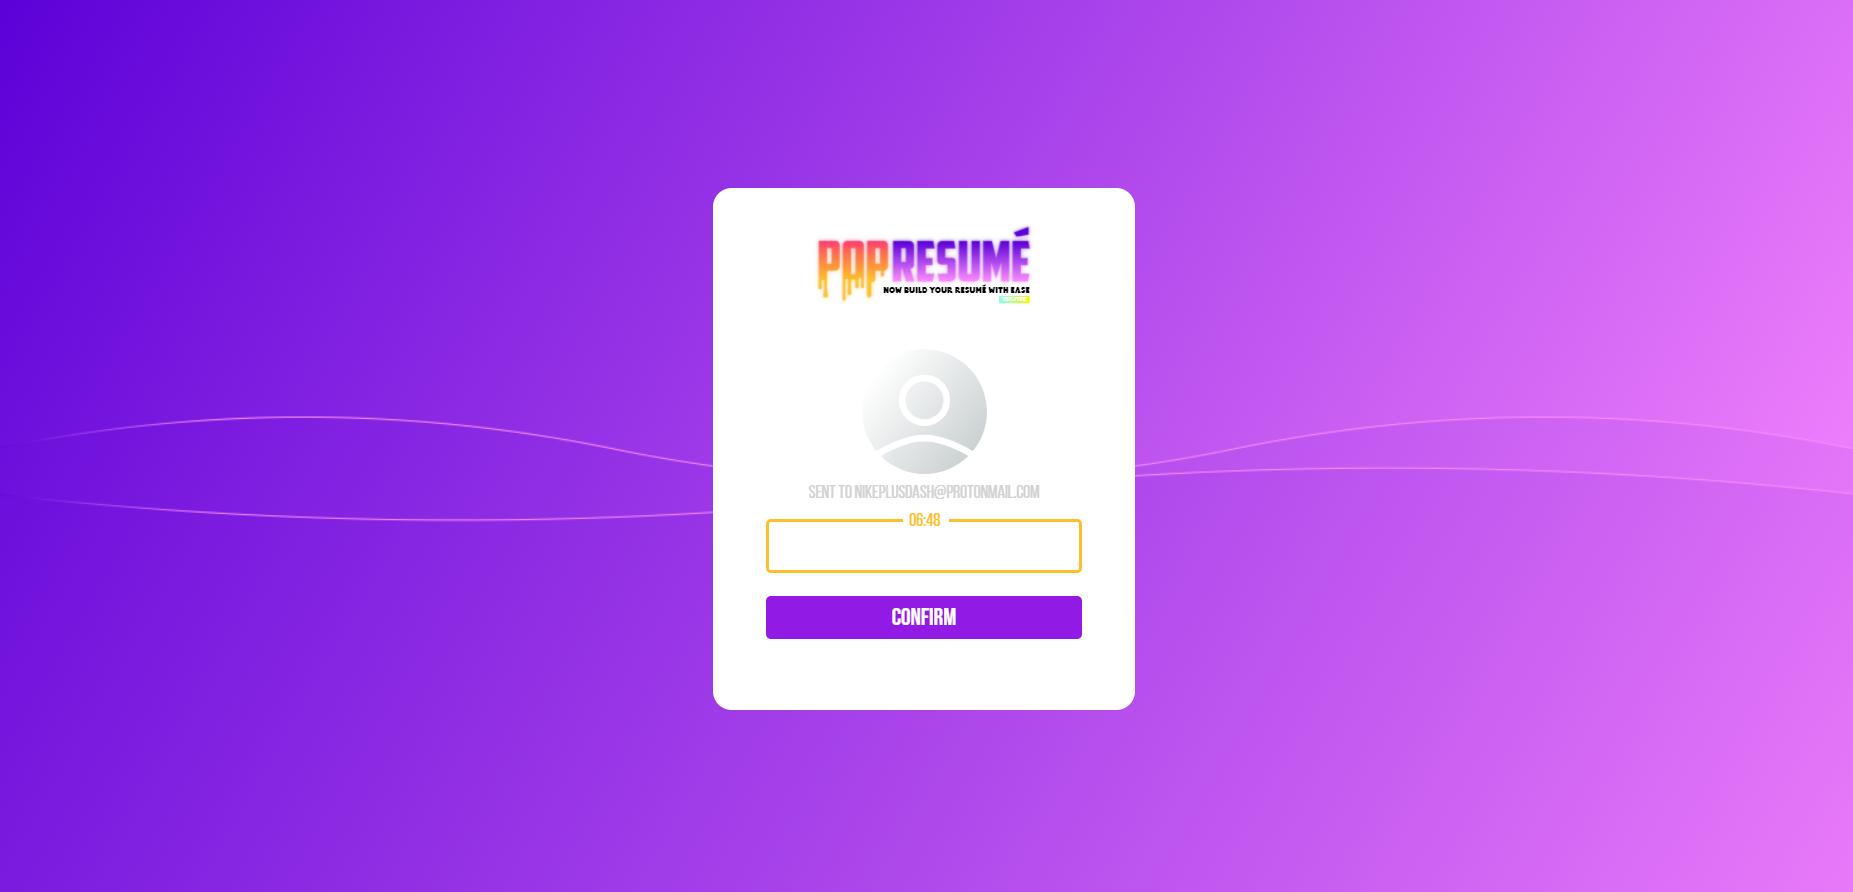
\includegraphics[width=\linewidth]{Screenshot 2021-06-07 051626.png}
        \caption{OTP}
    \end{minipage}
\end{figure}
\begin{figure}[H]
\centering
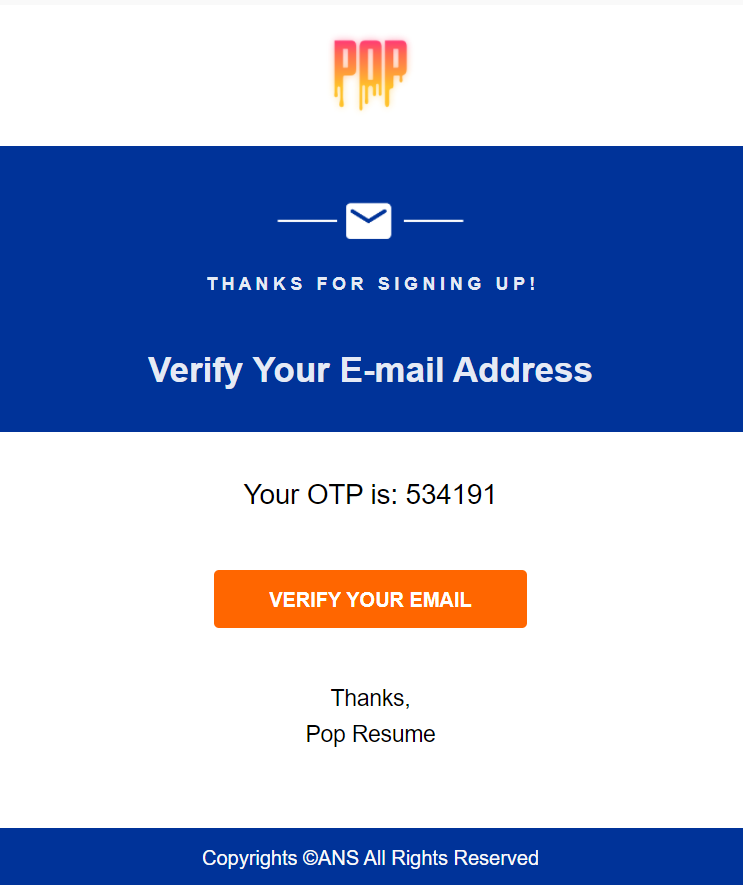
\includegraphics[width=0.5\linewidth]{Screenshot 2021-06-07 051656.png}
\caption{Mail Preview}
\end{figure}

\begin{figure}[H]
    \begin{minipage}{0.47\textwidth}
        \centering
        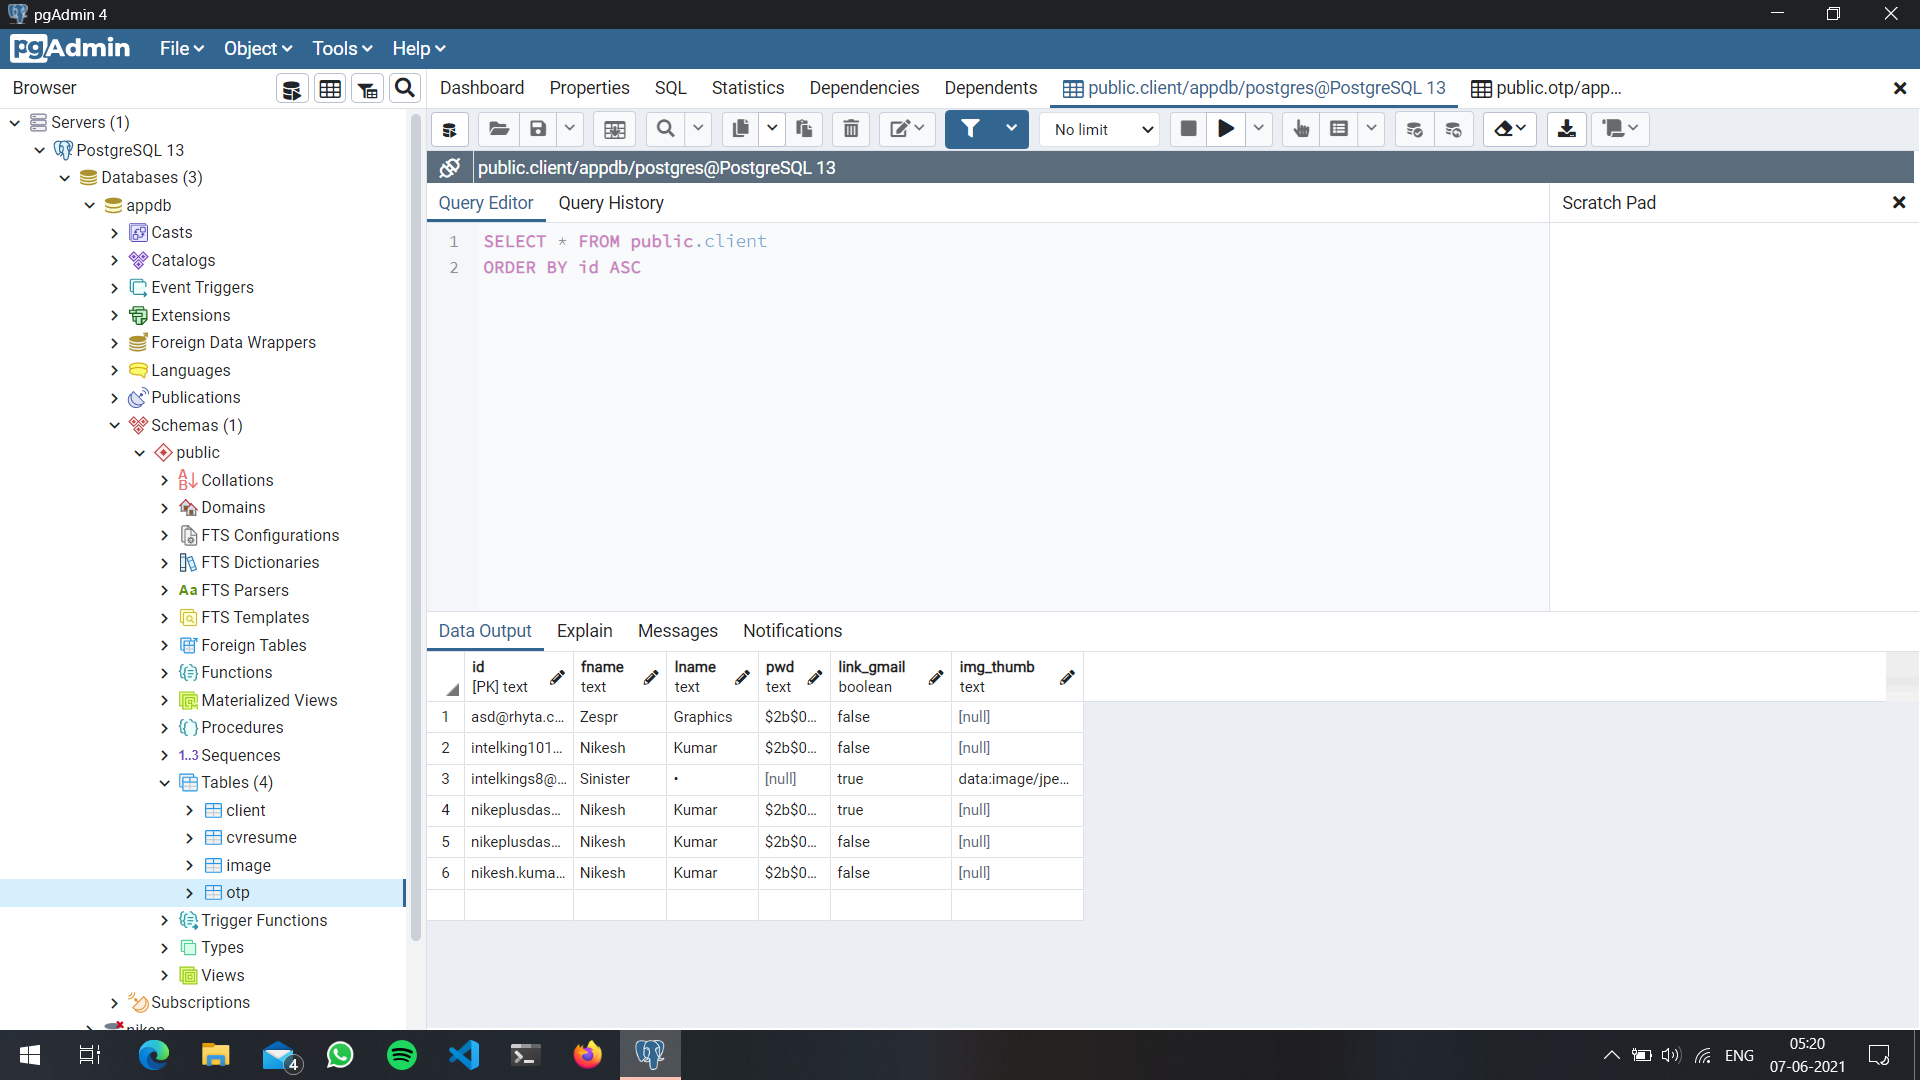
\includegraphics[width=\linewidth]{Screenshot (131).png}
        \caption{Backend Entries for Users}
    \end{minipage}\hfill
    \begin{minipage}{0.47\textwidth}
        \centering
        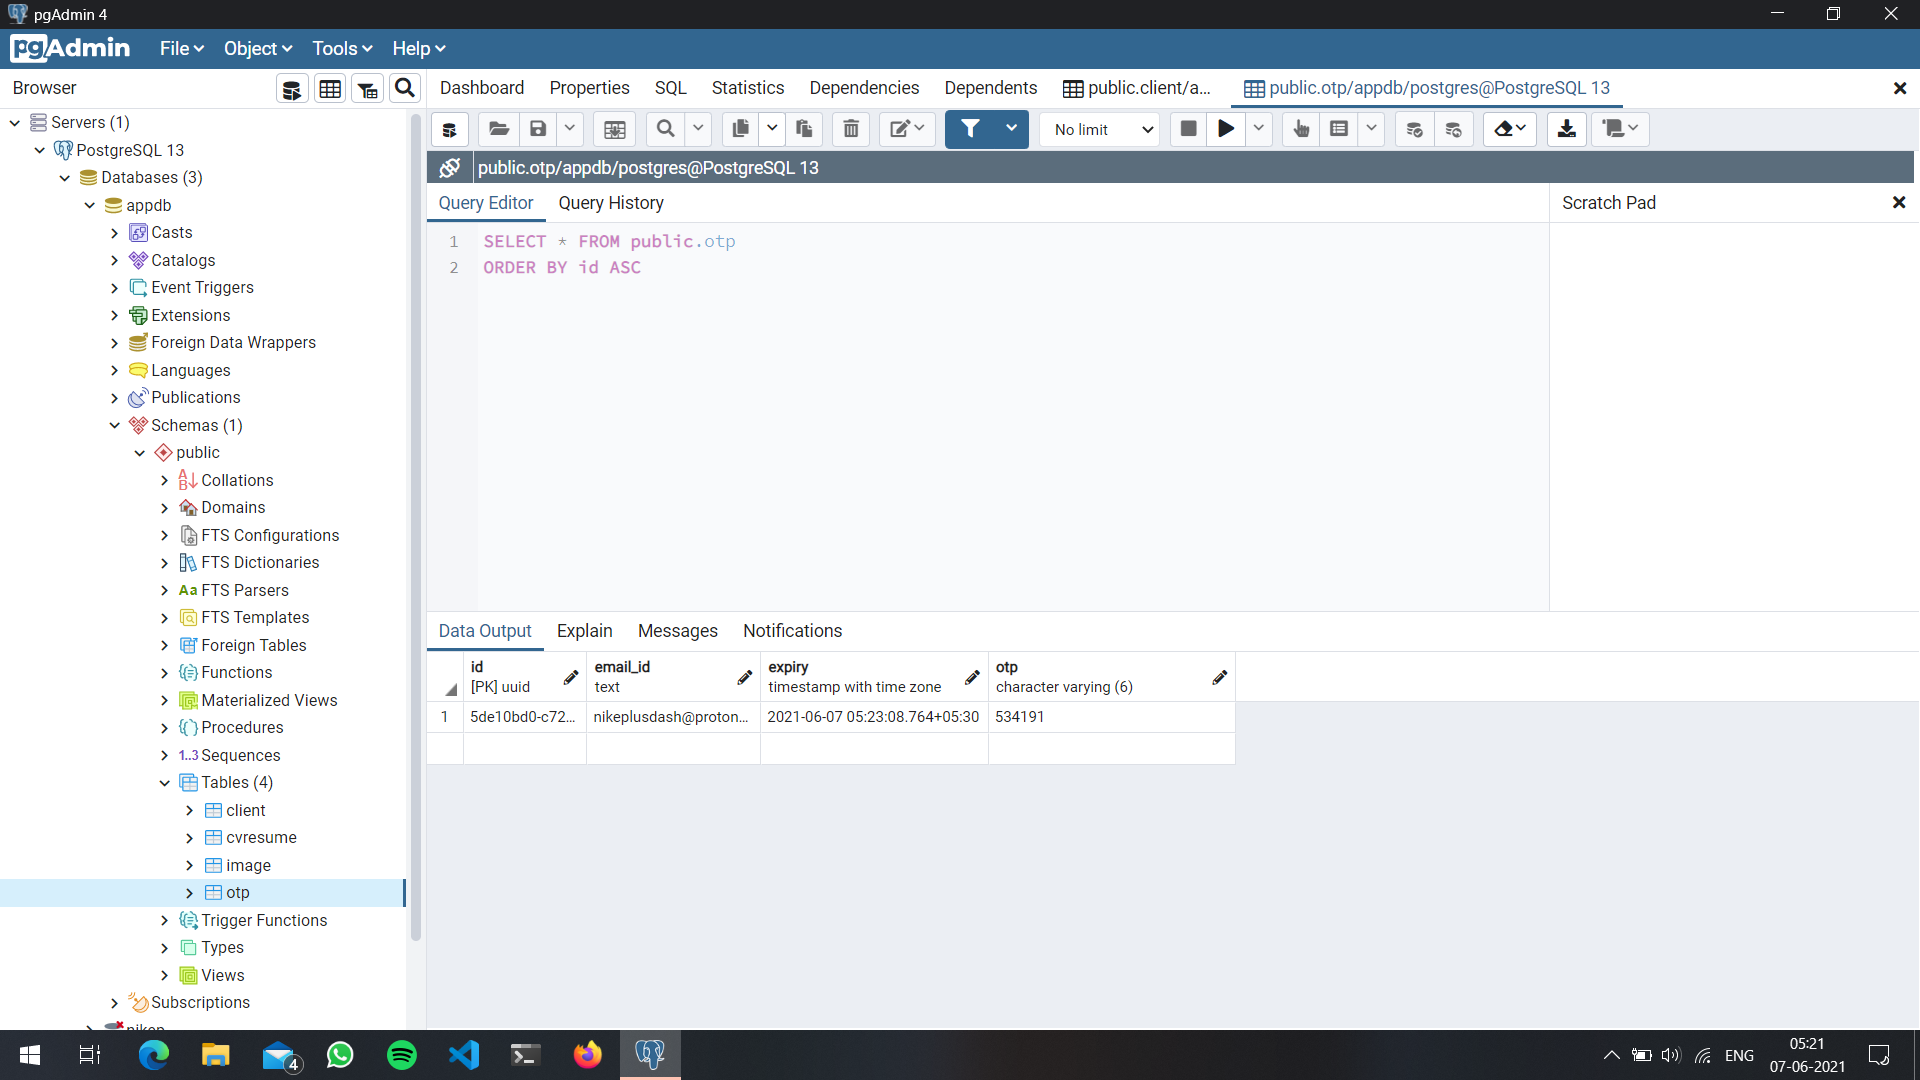
\includegraphics[width=\linewidth]{Screenshot (132).png}
        \caption{Backend Entries for OTP}
    \end{minipage}
\end{figure}
\begin{figure}[H]
\centering
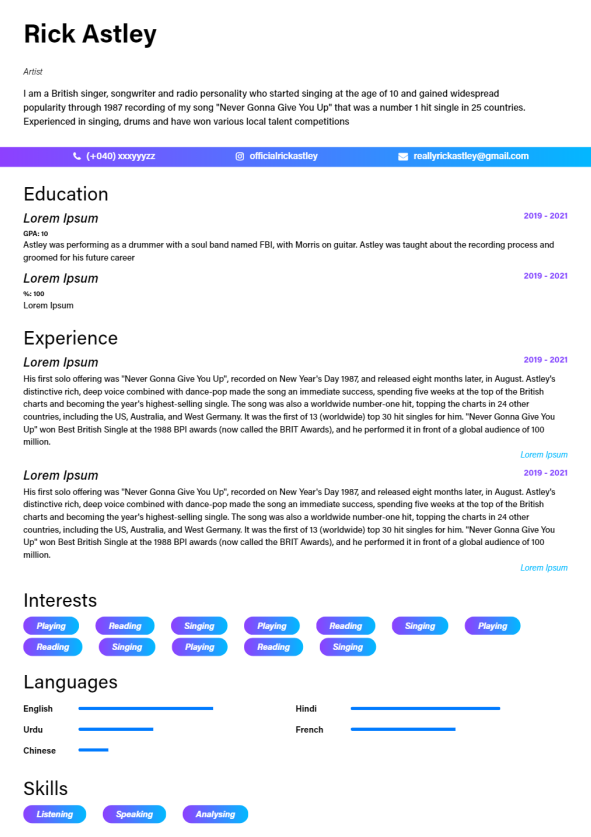
\includegraphics[width=0.74\linewidth]{SamplePDF.png}
\caption{PDF Preview}
\end{figure}

\begin{figure}[H]
\centering
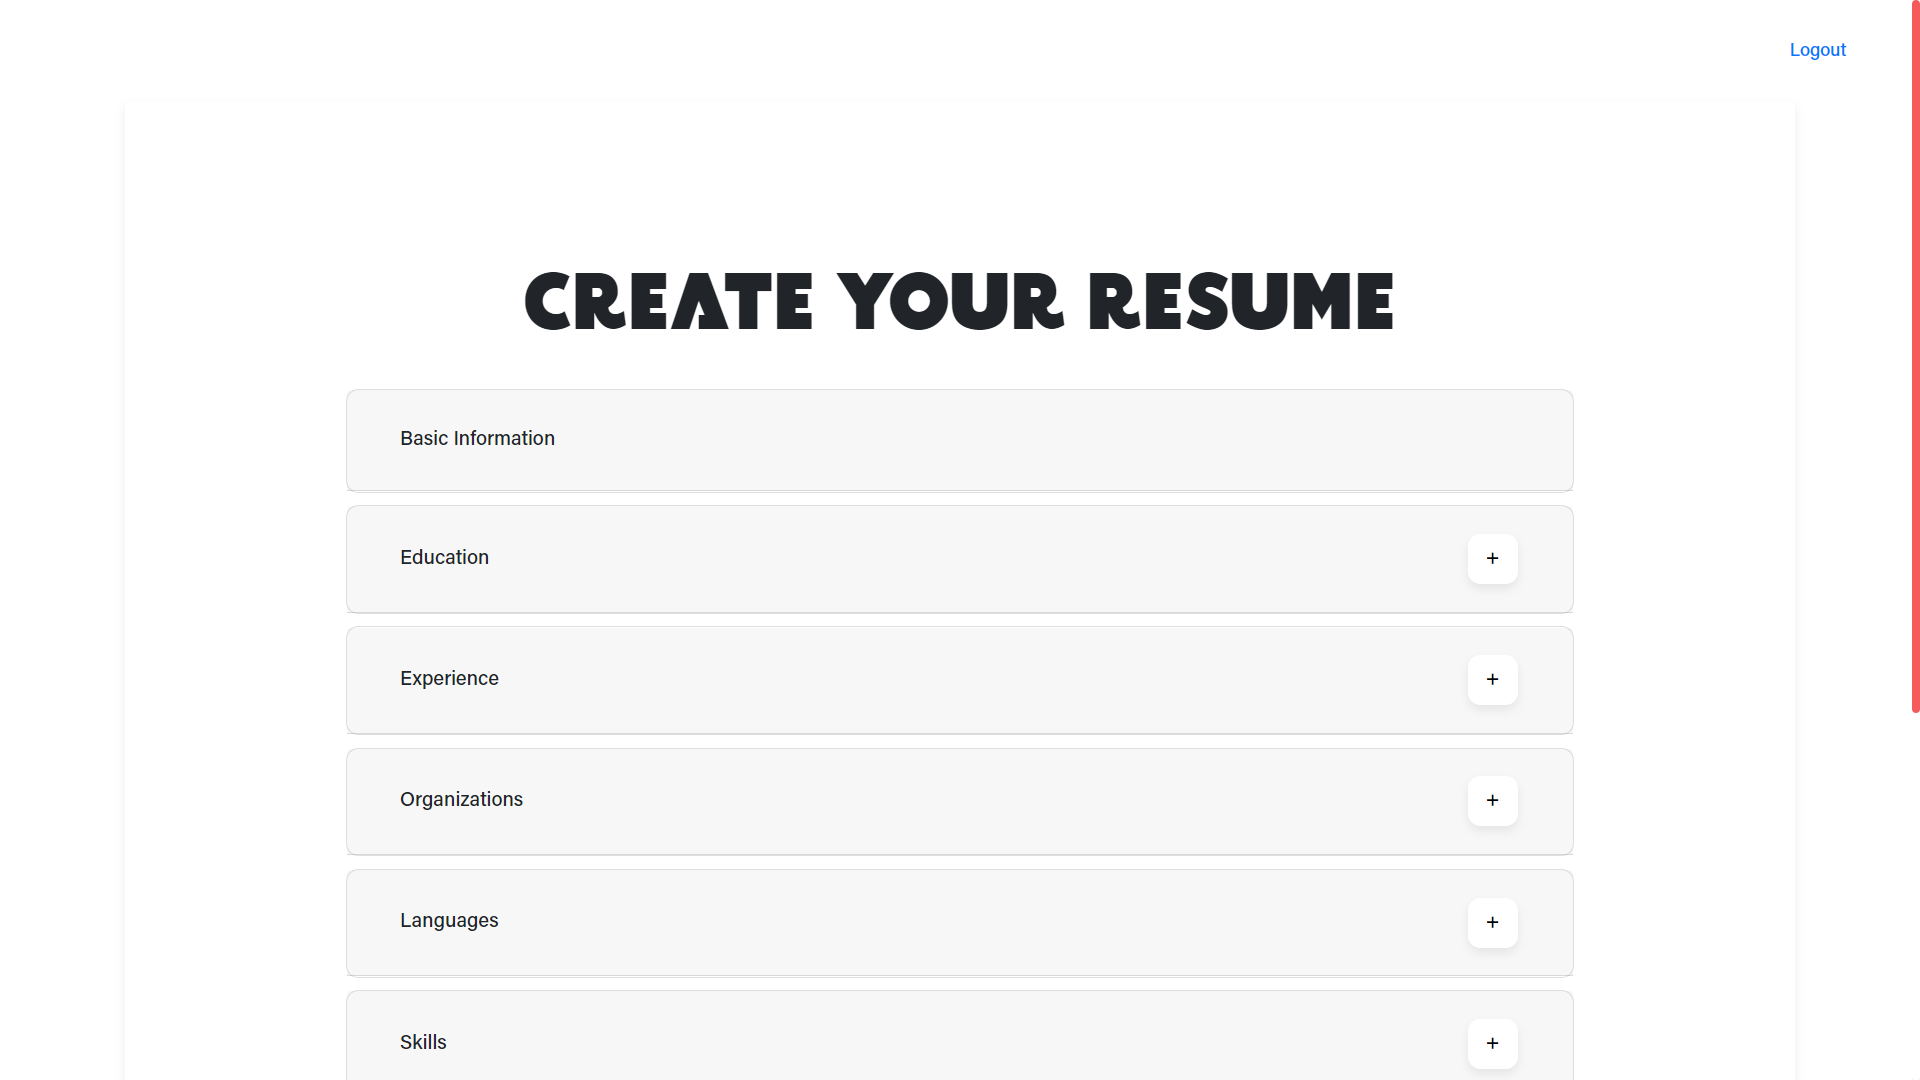
\includegraphics[width=0.74\linewidth]{Screenshot (134).png}
\caption{Resume Building Page}
\end{figure}
% \newpage

% ---------------- Conclusion ----------------
\section*{\LARGE{Conclusion}}
\addcontentsline{toc}{section}{\protect\numberline{}Conclusion}
This App aims to develop a resume platform that allows users to register and create themed resumes with ease because we believe a good resume can provide a user an edge when compared to other candidates for the same role. The web application boasts of a minimalistic, yet attractive and easily navigable user interface, and users can generate neat and professional resumes without any hassle. 
% \newpage

% ---------------- Future Work ----------------
\section*{\LARGE{Future Work}}
\addcontentsline{toc}{section}{\protect\numberline{}Future Work}
{\justify
Possible extensions to the app are feasible

\begin{itemize}
\item Add more resume templates
\item A dashboard for all resume
\item Improve security
\item Real-time editability
\end{itemize}
}

% \newpage

% ---------------- References ----------------
% \section*{\LARGE{References}}
% \addcontentsline{toc}{section}{\protect\numberline{}References}
% \begin{thebibliography}{widest entry} 
% \bibitem[1]{picasso} \url{https://square.github.io/picasso/}
% \bibitem[2]{dotsindicator} \url{https://github.com/tommybuonomo/dotsindicator}
% \bibitem[3]{bubbletab} \url{https://github.com/akshay2211/BubbleTabBar}
% \bibitem[4]{cardstack} \url{https://github.com/loopeer/CardStackView}
% \bibitem[5]{firebase} \url{https://firebase.google.com/}
% \end{thebibliography}   

\end{document}